%
% Ne pas compiler si pas de sagemath. Voir results.pdf alors
%
\documentclass{article}
\usepackage{graphicx}
\usepackage{amssymb,amsmath}
\usepackage{hyperref}
\usepackage[latin1]{inputenc}
\usepackage{enumitem}
\usepackage{sagetex} % requires sagemath
\usepackage{mathabx}
\usepackage{dsfont}
\usepackage{float}
\usepackage[ruled]{algorithm}
\usepackage{algorithmicx}
\usepackage[noend]{algpseudocode}
\algrenewcommand{\algorithmiccomment}[1]{\hfill \# {\scriptsize #1}} 
\algnewcommand\algorithmicinput{\textbf{Input:}}
\algnewcommand\Input{\item[\algorithmicinput]}
\algnewcommand\algorithmicoutput{\textbf{Output:}}
\algnewcommand\Output{\item[\algorithmicoutput]}
\algnewcommand\algodesc{\textbf{Description:}}
\algnewcommand\Desc{\item[\algodesc]}
\algnewcommand\algouse{\textbf{Usage:}}
\algnewcommand\Use{\item[\algouse]}
\newcommand{\be}{\begin{eqnarray*}}
\newcommand{\ee}{\end{eqnarray*}}
\newcommand{\ben}{\begin{eqnarray}}
\newcommand{\een}{\end{eqnarray}}
\newcommand{\dsp}{\displaystyle}
\makeatletter
\newcommand{\algrule}[1][.2pt]{\par\vskip.5\baselineskip\hrule height #1\par\vskip.5\baselineskip}
\makeatother
\DeclareMathOperator\erf{erf}
\def\E{\mathbb{E}}
\def\R{\mathbb{R}}
\def\Tmin{T_{\min}}
\def\Tmax{T^{\max}}
\def\mzero{\widehat{m}_0}
\usepackage{array}
\usepackage[justification=centering]{caption}
%\usepackage{showframe}
\newcolumntype{P}[1]{>{\centering\arraybackslash}p{#1}}
\begin{document}
Remarques g�n�rales:
\begin{itemize}
\item Le vecteur low n'a pas �t� pris en compte dans le temps calcul de G
\item Ici la derni�re version V2 est faite en C++ avec armadillo. L'interfa�age avec R (RcppArmadillo) semble donner des temps comparables � C++  armadillo.
\item Les mesures ont �t� faites sur math11 - elles sont relatives car d'autres utilisateurs pouvaient l'utiliser en m�me temps
\item Le temps calcul pour neuro-stat regroupe les temps calcul de $G$, $\mu_1$, $\mu_2$ et $\mu_A$
\item La version PWC est ma version C++ armadillo avec les fonctions constantes par morceaux
%\item Dans le tableau, l'erreur entre NeuroCorr et la derni�re version est assez grande pour les 2 derniers exemples (1e-5)
\end{itemize}

\section{50 et 300 spikes sur l'intervalle de temps $]0,8]$}
\begin{itemize}
\item $\delta=0.02$, $K=5$ (donc $A=0.1$)
\item $]\Tmin,\Tmax]=]0,8]$
\item Environ 6 et 37 spikes par unit� de temps
\end{itemize}
\begin{sagesilent}
Gns = {10: 0.023, 50: 0.433, 100: 1.329, 200 : 5.444, 500: 33.811, 1000: 135.266}
G = {10: 0.0039635, 50: 0.0563278, 100: 0.186973, 200 : 0.606324, 500: 5.61699, 1000: 29.2367}
b = {10: 0.000452239, 50: 0.00623007, 100: 0.0189842, 200 : 0.0585475, 500: 0.381913, 1000: 1.64153}
bpw = {10: 0.0103129, 50: 0.166311, 100: 0.51991, 200 : 2.04569, 500: 12.9949, 1000: 52.0342}
b_300 = {100: 0.0735659, 1000: 7.86702}
#G_300 = {100: 0.706314, 1000: 132.815}
G_300 = {100: 0.74474, 1000: 141.065}
Gk = {10: 0.0057983, 50: 0.0879065, 100: 0.253229, 200 : 1.00483, 500: 7.87857, 1000: 37.1691}
#Gk_300 = {100: 1.20614, 1000: 171.009}
Gk_300 = {100: 1.2538, 1000: 167.171}
Gpw = {10: 0.0260233, 50: 0.354829, 100: 1.11726, 200 : 4.45412, 500: 27.913, 1000: 111.757}
bpw_300 = {100: 6.91051, 1000: 668.701}
#Gpw_300 = {100: 6.67172, 1000: 628.077}
Gpw_300 = {100: 6.91094, 1000: 628.263}
#Gns_300 = {100: 2.977, 1000: 294.479}
Gns_300 = {100: 3.042, 1000: 325.881}
errGGk = {10: 9.99201e-16, 50: 1.11022e-15, 100: 1.11022e-15, 200 : 1.11022e-15, 500: 1.11022e-15, 1000: 1.11022e-15}
errGGpw = {10: 3.9968e-15, 50: 3.9968e-15, 100: 3.9968e-15, 200 : 1.02141e-14, 500: 1.02141e-14, 1000: 1.02141e-14}
errGGns = {10: 2.9976e-15, 50: 3.10862e-15, 100: 3.9968e-15, 200 : 1.02141e-14, 500: 1.02141e-14, 1000: 1.02141e-14}
errGpwGns = {10: 1.9984e-15, 50: 3.10862e-15, 100: 3.10862e-15, 200 : 3.9968e-15, 500: 9.76996e-15, 1000:  9.76996e-15}
#errGGns_300 = {100: 3.1244e-05, 1000: 3.5299e-05}
errGGns_300 = {100: 4.20108e-13, 1000: 4.60076e-13}
#errGGk_300 = {100: 1.02141e-14, 1000: 1.02141e-14}
errGGk_300 = {100: 0 , 1000: 0}
#errGGpw_300 = {100:  3.10862e-13, 1000: 3.28626e-13}
errGGpw_300 = {100: 3.10862e-13 , 1000: 3.30402e-13}
#errGpwGns_300 = {100: 3.1244e-05, 1000: 3.5299e-05}
errGpwGns_300 = {100: 3.79696e-13, 1000: 5.00933e-13}
#######
######
Gns_K9 = {10: 0.0110000000000241, 50: 0.262, 100: 1.02099999999999, 200 : 3.96899999999999, 500: 24.92, 1000: 99.897}
G_K9 = {10: 0.000583405, 50: 0.0119562, 100: 0.0480052, 200 : 0.188212, 500: 2.16265, 1000: 11.107}
b_K9 = {10: 6.726e-05, 50: 0.00130105, 100: 0.00510349, 200 : 0.0195296, 500: 0.120961, 1000: 0.731615 }
bpw_K9 = {10: 0.0155135, 50: 0.361674, 100: 1.44294, 200 : 5.7283, 500: 36.0034, 1000: 143.201 }
Gk_K9 = {10: 0.00103257, 50: 0.0207153, 100: 0.0791348, 200 : 0.305313, 500: 2.71521, 1000: 13.0226 }
Gpw_K9 = {10: 0.0220048, 50: 0.491713, 100: 1.98809, 200 : 7.89035, 500: 49.4951, 1000: 197.95 }
errGGk_K9 = {10: 0, 50: 0, 100: 0, 200 : 0, 500: 0, 1000: 0}
errGGpw_K9 = {10: 1.50102e-13, 50: 1.50102e-13, 100: 1.70086e-13, 200 : 1.70086e-13, 500: 1.70086e-13, 1000: 1.70086e-13}
errGGns_K9 = {10: 1.19904e-13, 50: 1.19904e-13, 100: 1.19904e-13, 200 : 1.19904e-13, 500: 1.20126e-13, 1000: 1.20348e-13}
errGpwGns_K9 = {10: 5.9952e-14, 50: 6.03961e-14, 100: 6.03961e-14, 200 : 7.01661e-14, 500: 7.01661e-14, 1000: 7.01661e-14}
\end{sagesilent}
\begin{table}[H]
\resizebox{\textwidth}{!}{
  {\renewcommand{\arraystretch}{1.2}
  \begin{tabular}{|P{2.45cm}|P{1.5cm}|P{1.15cm}|P{1.3cm}|P{1.15cm}|P{1.1cm}|P{1.1cm}|P{1.1cm}|P{1.1cm}|}
\hline
Temps en secondes (ou erreur) ------------------- nb de neurones   & NeuroCorr (neuro-stat). Total (Gns) & Version V2 (sans $k_1$, $k_2$). matrice G & Version V2 (avec $k_1$, $k_2$). matrice Gk & Version PWC. matrice Gpw & Erreur {\small{$\|G-Gk\|_{\infty}$}} & Erreur {\small{$\|G-Gpw\|_{\infty}$}} & Erreur {\small{$\|G-Gns\|_{\infty}$}} & Erreur {\small{$\|Gpw-Gns\|_{\infty}$}} \\
\hline
\hline
{\small{M=10 ($\simeq$50 spikes/neurone)}}&  $\sage{"{0:.2f}".format(float(Gns[10]))}$ & $\sage{"{0:.2f}".format(float(G[10]))}$ & $\sage{"{0:.2f}".format(float(Gk[10]))}$ & $\sage{"{0:.2f}".format(float(Gpw[10]))}$ & $\sage{"{0:.2g}".format(float(errGGk[10]))}$ &$\sage{"{0:.2g}".format(float(errGGpw[10]))}$ &$\sage{"{0:.2g}".format(float(errGGns[10]))}$&$\sage{"{0:.2g}".format(float(errGpwGns[10]))}$ \\
\hline
{\small{M=50 ($\simeq$50 spikes/neurone)}}&  $\sage{"{0:.2f}".format(float(Gns[50]))}$ & $\sage{"{0:.2f}".format(float(G[50]))}$ & $\sage{"{0:.2f}".format(float(Gk[50]))}$ & $\sage{"{0:.2f}".format(float(Gpw[50]))}$ & $\sage{"{0:.2g}".format(float(errGGk[50]))}$ &$\sage{"{0:.2g}".format(float(errGGpw[50]))}$ &$\sage{"{0:.2g}".format(float(errGGns[50]))}$&$\sage{"{0:.2g}".format(float(errGpwGns[50]))}$\\
\hline
{\small{M=100 ($\simeq$50 spikes/neurone)}}&  $\sage{"{0:.2f}".format(float(Gns[100]))}$ & $\sage{"{0:.2f}".format(float(G[100]))}$ & $\sage{"{0:.2f}".format(float(Gk[100]))}$ & $\sage{"{0:.2f}".format(float(Gpw[100]))}$  & $\sage{"{0:.2g}".format(float(errGGk[100]))}$ &$\sage{"{0:.2g}".format(float(errGGpw[100]))}$ &$\sage{"{0:.2g}".format(float(errGGns[100]))}$&$\sage{"{0:.2g}".format(float(errGpwGns[100]))}$\\
\hline
{\small{M=200 ($\simeq$50 spikes/neurone)}}&  $\sage{"{0:.2f}".format(float(Gns[200]))}$ & $\sage{"{0:.2f}".format(float(G[200]))}$ & $\sage{"{0:.2f}".format(float(Gk[200]))}$ & $\sage{"{0:.2f}".format(float(Gpw[200]))}$  & $\sage{"{0:.2g}".format(float(errGGk[200]))}$ &$\sage{"{0:.2g}".format(float(errGGpw[200]))}$ &$\sage{"{0:.2g}".format(float(errGGns[200]))}$&$\sage{"{0:.2g}".format(float(errGpwGns[200]))}$\\
\hline
{\small{M=500 ($\simeq$50 spikes/neurone)}}&  $\sage{"{0:.2f}".format(float(Gns[500]))}$ & $\sage{"{0:.2f}".format(float(G[500]))}$ & $\sage{"{0:.2f}".format(float(Gk[500]))}$ & $\sage{"{0:.2f}".format(float(Gpw[500]))}$ & $\sage{"{0:.2g}".format(float(errGGk[500]))}$ &$\sage{"{0:.2g}".format(float(errGGpw[500]))}$ &$\sage{"{0:.2g}".format(float(errGGns[500]))}$&$\sage{"{0:.2g}".format(float(errGpwGns[500]))}$\\
\hline
{\small{M=1000 ($\simeq$50 spikes/neurone)}}&  $\sage{"{0:.2f}".format(float(Gns[1000]))}$ & $\sage{"{0:.2f}".format(float(G[1000]))}$ & $\sage{"{0:.2f}".format(float(Gk[1000]))}$ & $\sage{"{0:.2f}".format(float(Gpw[1000]))}$ & $\sage{"{0:.2g}".format(float(errGGk[1000]))}$ &$\sage{"{0:.2g}".format(float(errGGpw[1000]))}$ &$\sage{"{0:.2g}".format(float(errGGns[1000]))}$&$\sage{"{0:.2g}".format(float(errGpwGns[1000]))}$\\
\hline
%{\small{M=100 ($\simeq$300 spikes/neurone)}}&  $\sage{"{0:.2f}".format(float(Gns_300[100]))}$ & $\sage{"{0:.2f}".format(float(G_300[100]))}$ & $\sage{"{0:.2f}".format(float(Gk_300[100]))}$ & $\sage{"{0:.2f}".format(float(Gpw_300[100]))}$ & $\sage{"{0:.2g}".format(float(errGGk_300[100]))}$ &$\sage{"{0:.2g}".format(float(errGGpw_300[100]))}$ &$\sage{"{0:.2g}".format(float(errGGns_300[100]))}$&$\sage{"{0:.2g}".format(float(errGpwGns_300[100]))}$\\
\hline
%{\small{M=1000 ($\simeq$300 spikes/neurone)}}&  $\sage{"{0:.2f}".format(float(Gns_300[1000]))}$ & $\sage{"{0:.2f}".format(float(G_300[1000]))}$ & $\sage{"{0:.2f}".format(float(Gk_300[1000]))}$ & $\sage{"{0:.2f}".format(float(Gpw_300[1000]))}$ & $\sage{"{0:.2g}".format(float(errGGk_300[1000]))}$ &$\sage{"{0:.2g}".format(float(errGGpw_300[1000]))}$ &$\sage{"{0:.2g}".format(float(errGGns_300[1000]))}$&$\sage{"{0:.2g}".format(float(errGpwGns_300[1000]))}$\\
{\small{M=100 ($\simeq$300 spikes/neurone)}}&  $\sage{"{0:.2f}".format(float(Gns_300[100]))}$ & $\sage{"{0:.2f}".format(float(G_300[100]))}$ & $\sage{"{0:.2f}".format(float(Gk_300[100]))}$ & $\sage{"{0:.2f}".format(float(Gpw_300[100]))}$ & $\sage{"{0:.2g}".format(float(errGGk_300[100]))}$ &$\sage{"{0:.2g}".format(float(errGGpw_300[100]))}$ &$\sage{"{0:.2g}".format(float(errGGns_300[100]))}$&$\sage{"{0:.2g}".format(float(errGpwGns_300[100]))}$\\
\hline
{\small{M=1000 ($\simeq$300 spikes/neurone)}}&  $\sage{"{0:.2f}".format(float(Gns_300[1000]))}$ & $\sage{"{0:.2f}".format(float(G_300[1000]))}$ & $\sage{"{0:.2f}".format(float(Gk_300[1000]))}$ & $\sage{"{0:.2f}".format(float(Gpw_300[1000]))}$ & $\sage{"{0:.2g}".format(float(errGGk_300[1000]))}$ &$\sage{"{0:.2g}".format(float(errGGpw_300[1000]))}$ &$\sage{"{0:.2g}".format(float(errGGns_300[1000]))}$&$\sage{"{0:.2g}".format(float(errGpwGns_300[1000]))}$\\
\hline
\end{tabular}}}
\caption{Temps de calcul pour $G$ - 6 et 37 spikes par seconde sur $]0,8]$}
\end{table}    

\section{750 spikes sur $]0,20]$}
\begin{itemize}
\item $\delta=0.02$, $K=5$ (donc $A=0.1$)
\item $]\Tmin,\Tmax]=]0,20]$
\item Environ 37 spikes par unit� de temps
\item La version PWC est tr�s longue, les r�sultats ne sont pas montr�s ici
\end{itemize}
%%%%%%%%%%%%%%%
%%%%%% G - 750 spikes 
%%%%%%%%%%%%%%%
\begin{sagesilent}
load('results/times750.sage')
load('results/timesR750.sage')
load('results/error750.sage')
bns=Gns
\end{sagesilent}
\begin{table}[H]
\resizebox{\textwidth}{!}{
  {\renewcommand{\arraystretch}{1.2}
  \begin{tabular}{|P{2.45cm}|P{1.5cm}|P{1.15cm}|P{1.15cm}|P{1.1cm}|P{1.1cm}|}
\hline
Temps en secondes (ou erreur) ------------------- nb de neurones  & NeuroCorr (neuro-stat). Total (Gns) & Version V2 (sans $k_1$, $k_2$). matrice G & Version V2 (avec $k_1$, $k_2$). matrice Gk & Erreur {\small{$\|G-Gk\|_{\infty}$}}  & Erreur {\small{$\|G-Gns\|_{\infty}$}}  \\
\hline
\hline
{\small{M=10}}&  $\sage{"{0:.2f}".format(float(Gns[10]))}$ & $\sage{"{0:.2f}".format(float(G[10]))}$ & $\sage{"{0:.2f}".format(float(Gk[10]))}$  & $\sage{"{0:.2g}".format(float(errGGk[10]))}$  &$\sage{"{0:.2g}".format(float(errGGns[10]))}$ \\
\hline
{\small{M=50}}&  $\sage{"{0:.2f}".format(float(Gns[50]))}$ & $\sage{"{0:.2f}".format(float(G[50]))}$ & $\sage{"{0:.2f}".format(float(Gk[50]))}$  & $\sage{"{0:.2g}".format(float(errGGk[50]))}$  &$\sage{"{0:.2g}".format(float(errGGns[50]))}$\\
\hline
{\small{M=100}}&  $\sage{"{0:.2f}".format(float(Gns[100]))}$ & $\sage{"{0:.2f}".format(float(G[100]))}$ & $\sage{"{0:.2f}".format(float(Gk[100]))}$  & $\sage{"{0:.2g}".format(float(errGGk[100]))}$  &$\sage{"{0:.2g}".format(float(errGGns[100]))}$\\
\hline
{\small{M=200}}&  $\sage{"{0:.2f}".format(float(Gns[200]))}$ & $\sage{"{0:.2f}".format(float(G[200]))}$ & $\sage{"{0:.2f}".format(float(Gk[200]))}$   & $\sage{"{0:.2g}".format(float(errGGk[200]))}$  &$\sage{"{0:.2g}".format(float(errGGns[200]))}$\\
\hline
{\small{M=500}}&  $\sage{"{0:.2f}".format(float(Gns[500]))}$ & $\sage{"{0:.2f}".format(float(G[500]))}$ & $\sage{"{0:.2f}".format(float(Gk[500]))}$  & $\sage{"{0:.2g}".format(float(errGGk[500]))}$  &$\sage{"{0:.2g}".format(float(errGGns[500]))}$\\
\hline
{\small{M=1000}}&  $\sage{"{0:.2f}".format(float(Gns[1000]))}$ & $\sage{"{0:.2f}".format(float(G[1000]))}$ & $\sage{"{0:.2f}".format(float(Gk[1000]))}$  & $\sage{"{0:.2g}".format(float(errGGk[1000]))}$  &$\sage{"{0:.2g}".format(float(errGGns[1000]))}$\\
\hline
\end{tabular}}}
\caption{Temps de calcul pour $G$ - 37 spikes par seconde - $]0,20]$}
\end{table}    
%%%%%%%%%%%%%%%
%%%%%% b - 750 spikes 
%%%%%%%%%%%%%%%
\begin{table}[H]
\vspace*{-.8cm}
  \begin{center}
  \resizebox{.8\textwidth}{!}{
  {\renewcommand{\arraystretch}{1.2}
  \begin{tabular}{|P{2.45cm}|P{1.5cm}|P{1.3cm}|P{1.15cm}|P{1.1cm}|P{1.1cm}|P{1.1cm}|}
\hline
Temps en secondes (ou erreur) ------------------------- nb de neurones    & NeuroCorr (neuro-stat). Total (bns) & Version V2  matrice b   & Erreur {\small{$\|b-bns\|_{\infty}$}}  \\
\hline
\hline
{\small{M=10}}&  $\sage{"{0:.2f}".format(float(bns[10]))}$ & $\sage{"{0:.2f}".format(float(b[10]))}$  &$\sage{"{0:.2g}".format(float(errbbns[10]))}$\\
\hline
{\small{M=50}}&  $\sage{"{0:.2f}".format(float(bns[50]))}$ & $\sage{"{0:.2f}".format(float(b[50]))}$   &$\sage{"{0:.2g}".format(float(errbbns[50]))}$\\
\hline
{\small{M=100}}&  $\sage{"{0:.2f}".format(float(bns[100]))}$ & $\sage{"{0:.2f}".format(float(b[100]))}  $    &$\sage{"{0:.2g}".format(float(errbbns[100]))}$\\
\hline
{\small{M=200}}&  $\sage{"{0:.2f}".format(float(bns[200]))}$ & $\sage{"{0:.2f}".format(float(b[200]))}$    &$\sage{"{0:.2g}".format(float(errbbns[200]))}$\\
\hline
{\small{M=500}}&  $\sage{"{0:.2f}".format(float(bns[500]))}$ & $\sage{"{0:.2f}".format(float(b[500]))}$    &$\sage{"{0:.2g}".format(float(errbbns[500]))}$\\
\hline
{\small{M=1000}}&  $\sage{"{0:.2f}".format(float(bns[1000]))}$ & $\sage{"{0:.2f}".format(float(b[1000]))}$  &$\sage{"{0:.2g}".format(float(errbbns[1000]))}$\\
\hline
\end{tabular}}}
\caption{Temps de calcul pour $b$ - 37 spikes par seconde - $]0,20]$}
\end{center}
\end{table}    
\clearpage
%%%%%%%%%%%%%%%
%%%%%% G - 125 spikes 
%%%%%%%%%%%%%%%
\section{125 spikes sur $]0,20]$}
\begin{itemize}
\item $\delta=0.02$, $K=5$ (donc $A=0.1$)
\item $]\Tmin,\Tmax]=]0,20]$
\item Environ 6 spikes par unit� de temps
\end{itemize}
\begin{sagesilent}
load('results/times125.sage')
load('results/timesR125.sage')
load('results/error125.sage')
bns=Gns
\end{sagesilent}
\begin{table}[H]
\resizebox{\textwidth}{!}{
  {\renewcommand{\arraystretch}{1.2}
  \begin{tabular}{|P{2.2cm}|P{1.5cm}|P{1.15cm}|P{1.3cm}|P{1.15cm}|P{1.1cm}|P{1.1cm}|P{1.1cm}|P{1.1cm}|}
\hline
Temps en secondes (ou erreur) ------------------------------------ nb de neurones    & NeuroCorr (neuro-stat). Total (Gns) & Version V2 (sans $k_1$, $k_2$). matrice G & Version V2 (avec $k_1$, $k_2$). matrice Gk & Version PWC. matrice Gpw & Erreur {\small{$\|G-Gk\|_{\infty}$}} & Erreur {\small{$\|G-Gpw\|_{\infty}$}} & Erreur {\small{$\|G-Gns\|_{\infty}$}} & Erreur {\small{$\|Gpw-Gns\|_{\infty}$}} \\
\hline
\hline
{\small{M=10}}&  $\sage{"{0:.2f}".format(float(Gns[10]))}$ & $\sage{"{0:.2f}".format(float(G[10]))}$ & $\sage{"{0:.2f}".format(float(Gk[10]))}$ & $\sage{"{0:.2f}".format(float(Gpw[10]))}$ & $\sage{"{0:.2g}".format(float(errGGk[10]))}$ &$\sage{"{0:.2g}".format(float(errGGpw[10]))}$ &$\sage{"{0:.2g}".format(float(errGGns[10]))}$&$\sage{"{0:.2g}".format(float(errGpwGns[10]))}$ \\
\hline
{\small{M=50}}&  $\sage{"{0:.2f}".format(float(Gns[50]))}$ & $\sage{"{0:.2f}".format(float(G[50]))}$ & $\sage{"{0:.2f}".format(float(Gk[50]))}$ & $\sage{"{0:.2f}".format(float(Gpw[50]))}$ & $\sage{"{0:.2g}".format(float(errGGk[50]))}$ &$\sage{"{0:.2g}".format(float(errGGpw[50]))}$ &$\sage{"{0:.2g}".format(float(errGGns[50]))}$&$\sage{"{0:.2g}".format(float(errGpwGns[50]))}$\\
\hline
{\small{M=100}}&  $\sage{"{0:.2f}".format(float(Gns[100]))}$ & $\sage{"{0:.2f}".format(float(G[100]))}$ & $\sage{"{0:.2f}".format(float(Gk[100]))}$ & $\sage{"{0:.2f}".format(float(Gpw[100]))}$  & $\sage{"{0:.2g}".format(float(errGGk[100]))}$ &$\sage{"{0:.2g}".format(float(errGGpw[100]))}$ &$\sage{"{0:.2g}".format(float(errGGns[100]))}$&$\sage{"{0:.2g}".format(float(errGpwGns[100]))}$\\
\hline
{\small{M=200}}&  $\sage{"{0:.2f}".format(float(Gns[200]))}$ & $\sage{"{0:.2f}".format(float(G[200]))}$ & $\sage{"{0:.2f}".format(float(Gk[200]))}$ & $\sage{"{0:.2f}".format(float(Gpw[200]))}$  & $\sage{"{0:.2g}".format(float(errGGk[200]))}$ &$\sage{"{0:.2g}".format(float(errGGpw[200]))}$ &$\sage{"{0:.2g}".format(float(errGGns[200]))}$&$\sage{"{0:.2g}".format(float(errGpwGns[200]))}$\\
\hline
{\small{M=500}}&  $\sage{"{0:.2f}".format(float(Gns[500]))}$ & $\sage{"{0:.2f}".format(float(G[500]))}$ & $\sage{"{0:.2f}".format(float(Gk[500]))}$ & $\sage{"{0:.2f}".format(float(Gpw[500]))}$ & $\sage{"{0:.2g}".format(float(errGGk[500]))}$ &$\sage{"{0:.2g}".format(float(errGGpw[500]))}$ &$\sage{"{0:.2g}".format(float(errGGns[500]))}$&$\sage{"{0:.2g}".format(float(errGpwGns[500]))}$\\
\hline
{\small{M=1000}}&  $\sage{"{0:.2f}".format(float(Gns[1000]))}$ & $\sage{"{0:.2f}".format(float(G[1000]))}$ & $\sage{"{0:.2f}".format(float(Gk[1000]))}$ & $\sage{"{0:.2f}".format(float(Gpw[1000]))}$ & $\sage{"{0:.2g}".format(float(errGGk[1000]))}$ &$\sage{"{0:.2g}".format(float(errGGpw[1000]))}$ &$\sage{"{0:.2g}".format(float(errGGns[1000]))}$&$\sage{"{0:.2g}".format(float(errGpwGns[1000]))}$\\
\hline
\end{tabular}}}
\caption{Temps de calcul pour $G$ - 6 spikes par seconde - $]0,20]$}
\end{table}    
%%%%%%%%%%%%%%%
%%%%%% b - 125 spikes 
%%%%%%%%%%%%%%%
\begin{table}[H]
\resizebox{\textwidth}{!}{
  {\renewcommand{\arraystretch}{1.2}
  \begin{tabular}{|P{2.2cm}|P{1.5cm}|P{1.3cm}|P{1.15cm}|P{1.1cm}|P{1.1cm}|P{1.1cm}|}
\hline
Temps en secondes (ou erreur) ------------------- nb de neurones    & NeuroCorr (neuro-stat). Total (bns) & Version V2  matrice b  & Version PWC. matrice $\mu_1$ &  Erreur {\small{$\|b-\mu_1\|_{\infty}$}} & Erreur {\small{$\|b-bns\|_{\infty}$}} & Erreur {\small{$\|\mu_1-bns\|_{\infty}$}} \\
\hline
\hline
{\small{M=10}}&  $\sage{"{0:.2f}".format(float(bns[10]))}$ & $\sage{"{0:.2f}".format(float(b[10]))}$  & $\sage{"{0:.2f}".format(float(mu[10]))}$ & $\sage{"{0:.2g}".format(float(errbmu[10]))}$ &$\sage{"{0:.2g}".format(float(errbbns[10]))}$&$\sage{"{0:.2g}".format(float(errbnsmu[10]))}$ \\
\hline
{\small{M=50}}&  $\sage{"{0:.2f}".format(float(bns[50]))}$ & $\sage{"{0:.2f}".format(float(b[50]))}$  & $\sage{"{0:.2f}".format(float(mu[50]))}$  &$\sage{"{0:.2g}".format(float(errbmu[50]))}$ &$\sage{"{0:.2g}".format(float(errbbns[50]))}$&$\sage{"{0:.2g}".format(float(errbnsmu[50]))}$\\
\hline
{\small{M=100}}&  $\sage{"{0:.2f}".format(float(bns[100]))}$ & $\sage{"{0:.2f}".format(float(b[100]))}$  & $\sage{"{0:.2f}".format(float(mu[100]))}$   &$\sage{"{0:.2g}".format(float(errbmu[100]))}$ &$\sage{"{0:.2g}".format(float(errbbns[100]))}$&$\sage{"{0:.2g}".format(float(errbnsmu[100]))}$\\
\hline
{\small{M=200}}&  $\sage{"{0:.2f}".format(float(bns[200]))}$ & $\sage{"{0:.2f}".format(float(b[200]))}$  & $\sage{"{0:.2f}".format(float(mu[200]))}$   &$\sage{"{0:.2g}".format(float(errbmu[200]))}$ &$\sage{"{0:.2g}".format(float(errbbns[200]))}$&$\sage{"{0:.2g}".format(float(errbnsmu[200]))}$\\
\hline
{\small{M=500}}&  $\sage{"{0:.2f}".format(float(bns[500]))}$ & $\sage{"{0:.2f}".format(float(b[500]))}$  & $\sage{"{0:.2f}".format(float(mu[500]))}$  &$\sage{"{0:.2g}".format(float(errbmu[500]))}$ &$\sage{"{0:.2g}".format(float(errbbns[500]))}$&$\sage{"{0:.2g}".format(float(errbnsmu[500]))}$\\
\hline
{\small{M=1000}}&  $\sage{"{0:.2f}".format(float(bns[1000]))}$ & $\sage{"{0:.2f}".format(float(b[1000]))}$  & $\sage{"{0:.2f}".format(float(mu[1000]))}$  &$\sage{"{0:.2g}".format(float(errbmu[1000]))}$ &$\sage{"{0:.2g}".format(float(errbbns[1000]))}$&$\sage{"{0:.2g}".format(float(errbnsmu[1000]))}$\\
\hline
\end{tabular}}}
\caption{Temps de calcul pour $b$ - 6 spikes par seconde - $]0,20]$}
\end{table}
\clearpage
\section{Intervalle $(0,600]$}
On consid�re l'intervalle de temps $(0,600]$ et $\displaystyle\sum_{i=1}^M\nu_i = 15000$. On a les r�sultats suivants:\\
\begin{table}[H]
\vspace*{-0.3cm}
  \begin{tabular}{|c|c|c|P{1.8cm}|P{2cm}|P{2cm}|P{2cm}|}
\hline
  M & $\nu$ & $\dsp\sum_{i=1}^M\nu_i$ & spike number per neuron on $(0,600]$& Elapsed time for $G$ (our method)& Elapsed time for $b$ (our method)& neuro-stat time \\
\hline
    100  & 150 & 15000 & 90000 &1243.33 &125.935 &1188.961\\
\hline
    200  & 75 & 15000 & 45000 &1247.23&128.933&2302.629\\
\hline
    500  & 30 & 15000 & 18000 &1998.98&129.578&5521.465\\
\hline
    1000  & 15 & 15000 & 9000 & 3049.78&190.101&10468.655\\
\hline
\end{tabular}
\caption{Temps calcul pour $\sum_{i=1}^M\nu_i=15000$}
\end{table}
\begin{minipage}{\textwidth}
  \begin{minipage}{.5\textwidth}
    \hspace*{-1.2cm}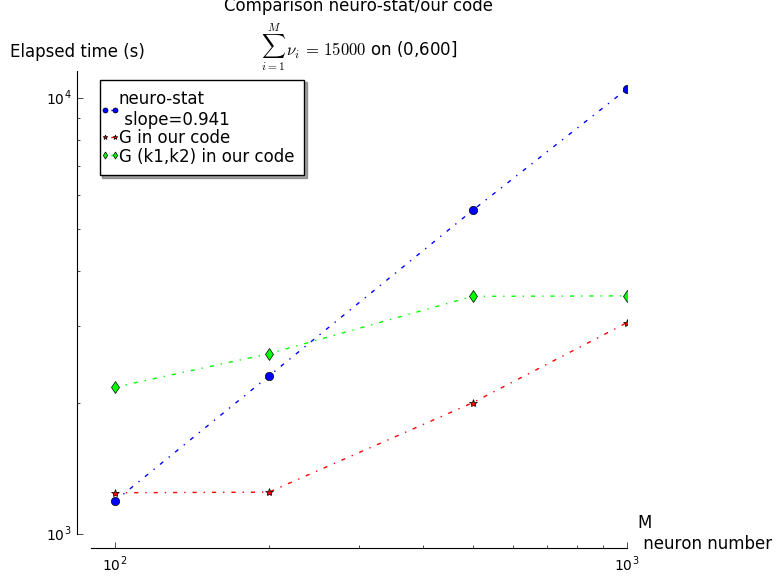
\includegraphics[width=1.4\textwidth]{figures/plot_times_15000.png}
\captionof{figure}{Comparaison des temps calcul pour $G$ (loglog)}
  \end{minipage}
    \begin{minipage}{.5\textwidth}
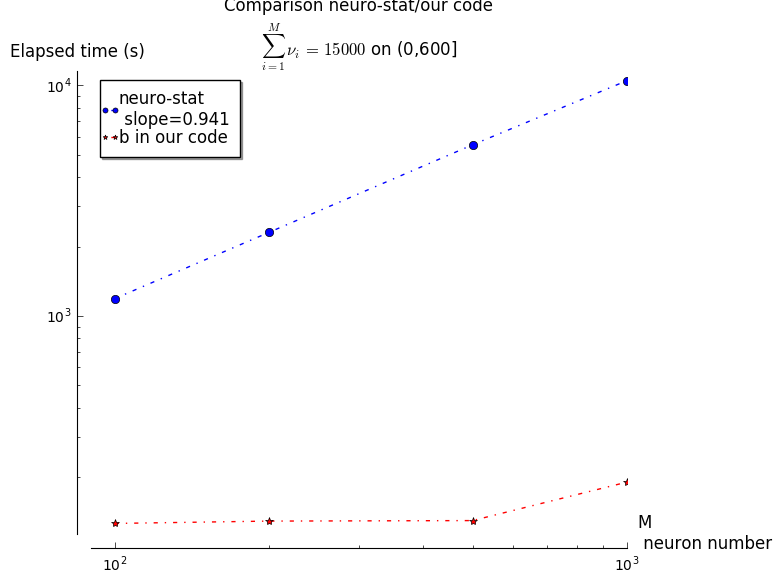
\includegraphics[width=1.4\textwidth]{figures/plot_times_b_15000.png}
\captionof{figure}{Comparaison des temps calcul pour $b$ (loglog)}
    \end{minipage}
    \end{minipage}


\begin{sagesilent}
load('results/error_15000.sage')
\end{sagesilent}
\begin{table}[H]
  \begin{tabular}{|c|P{1.8cm}|P{1.8cm}|P{1.8cm}|}
\hline
    nb de neurones & Erreur {\small{$\|G-Gns\|_{\infty}$}}  & Erreur {\small{$\|b-bns\|_{\infty}$}} & Erreur {\small{$\|G-Gk\|_{\infty}$}} \\
\hline
100 &$\sage{"{0:.2g}".format(float(errGGns[100]))}$ &$\sage{"{0:.2g}".format(float(errbbns[100]))}$&$\sage{"{0:.2g}".format(float(errGGk[100]))}$ \\
\hline
200 &$\sage{"{0:.2g}".format(float(errGGns[200]))}$ &$\sage{"{0:.2g}".format(float(errbbns[200]))}$&$\sage{"{0:.2g}".format(float(errGGk[200]))}$ \\
\hline
500 &$\sage{"{0:.2g}".format(float(errGGns[500]))}$ &$\sage{"{0:.2g}".format(float(errbbns[500]))}$&$\sage{"{0:.2g}".format(float(errGGk[500]))}$ \\
\hline
1000 &$\sage{"{0:.2g}".format(float(errGGns[1000]))}$ &$\sage{"{0:.2g}".format(float(errbbns[1000]))}$&$\sage{"{0:.2g}".format(float(errGGk[1000]))}$ \\
\hline
  \end{tabular}
\caption{Tableau des erreurs $\sum_{i=1}^M\nu_i=15000$}
\end{table}


    %%%% PARTIE A REPRENDRE (cas9 ?)
%%\begin{table}
%%\resizebox{\textwidth}{!}{
%%  {\renewcommand{\arraystretch}{1.2}
%%  \begin{tabular}{|P{2.6cm}|P{1.5cm}|P{1.3cm}|P{1.3cm}|P{1.3cm}|P{1cm}|P{1cm}|P{1cm}|P{1cm}|}
%%\hline
%%Temps en sec  & NeuroCorr (neuro-stat). Total (bns) & Version V2. Vecteur b & Version PWC. Vecteur bpw & Erreur $\|bns-b\|$ & Erreur $\|b-bpw\|$ & Erreur $\|bns-bpw\|$ \\
%%\hline
%%\hline
%%{\small{M=10 ($\simeq$50 spikes/neurone)}}&  $\sage{"{0:.2f}".format(float(Gns[10]))}$ & $\sage{"{0:.2f}".format(float(b[10]))}$  & $\sage{"{0:.2f}".format(float(bpw[10]))}$ & 0 & && \\
%%\hline
%%{\small{M=50 ($\simeq$50 spikes/neurone)}}&  $\sage{"{0:.2f}".format(float(Gns[50]))}$ & $\sage{"{0:.2f}".format(float(b[50]))}$  & $\sage{"{0:.2f}".format(float(bpw[50]))}$ & 0 & && \\
%%\hline
%%{\small{M=100 ($\simeq$50 spikes/neurone)}}&  $\sage{"{0:.2f}".format(float(Gns[100]))}$ & $\sage{"{0:.2f}".format(float(b[100]))}$  & $\sage{"{0:.2f}".format(float(bpw[100]))}$ & 0 & && \\
%%\hline
%%{\small{M=200 ($\simeq$50 spikes/neurone)}}&  $\sage{"{0:.2f}".format(float(Gns[200]))}$ & $\sage{"{0:.2f}".format(float(b[200]))}$  & $\sage{"{0:.2f}".format(float(bpw[200]))}$ & 0 & && \\
%%\hline
%%{\small{M=500 ($\simeq$50 spikes/neurone)}}&  $\sage{"{0:.2f}".format(float(Gns[500]))}$ & $\sage{"{0:.2f}".format(float(b[500]))}$  & $\sage{"{0:.2f}".format(float(bpw[500]))}$ & 0 & && \\
%%\hline
%%{\small{M=1000 ($\simeq$50 spikes/neurone)}}&  $\sage{"{0:.2f}".format(float(Gns[1000]))}$ & $\sage{"{0:.2f}".format(float(b[1000]))}$  & $\sage{"{0:.2f}".format(float(bpw[1000]))}$ & 0 & && \\
%%\hline
%%{\small{M=100 ($\simeq$300 spikes/neurone)}}&  $\sage{"{0:.2f}".format(float(Gns_300[100]))}$ & $\sage{"{0:.2f}".format(float(b_300[100]))}$  & $\sage{"{0:.2f}".format(float(bpw_300[100]))}$ & 0 & && \\
%%\hline
%%{\small{M=1000 ($\simeq$300 spikes/neurone)}}&  $\sage{"{0:.2f}".format(float(Gns_300[1000]))}$ & $\sage{"{0:.2f}".format(float(b_300[1000]))}$  & $\sage{"{0:.2f}".format(float(bpw_300[1000]))}$ & 0 & && \\
%%\hline
%%\end{tabular}}}
%%\end{table}    
%
%Intervalle de temps
%(0, 20]
%\begin{table}
%\resizebox{\textwidth}{!}{
%  {\renewcommand{\arraystretch}{1.2}
%  \begin{tabular}{|P{2.45cm}|P{1.5cm}|P{1.15cm}|P{1.3cm}|P{1.15cm}|P{1.1cm}|P{1.1cm}|P{1.1cm}|P{1.1cm}|}
%\hline
%Temps en secondes  & NeuroCorr (neuro-stat). Total (Gns) & Version V2 (sans $k_1$, $k_2$). matrice G & Version V2 (avec $k_1$, $k_2$). matrice Gk & Version PWC. matrice Gpw & Erreur {\small{$\|G-Gk\|_{\infty}$}} & Erreur {\small{$\|G-Gpw\|_{\infty}$}} & Erreur {\small{$\|G-Gns\|_{\infty}$}} & Erreur {\small{$\|Gpw-Gns\|_{\infty}$}} \\
%\hline
%\hline
%{\small{M=10 ($\simeq$50 spikes/neurone)}}&  $\sage{"{0:.2f}".format(float(Gns_K9[10]))}$ & $\sage{"{0:.2f}".format(float(G_K9[10]))}$ & $\sage{"{0:.2f}".format(float(Gk_K9[10]))}$ & $\sage{"{0:.2f}".format(float(Gpw_K9[10]))}$ & $\sage{"{0:.2g}".format(float(errGGk_K9[10]))}$ &$\sage{"{0:.2g}".format(float(errGGpw_K9[10]))}$ &$\sage{"{0:.2g}".format(float(errGGns_K9[10]))}$&$\sage{"{0:.2g}".format(float(errGpwGns_K9[10]))}$ \\
%\hline
%{\small{M=50 ($\simeq$50 spikes/neurone)}}&  $\sage{"{0:.2f}".format(float(Gns_K9[50]))}$ & $\sage{"{0:.2f}".format(float(G_K9[50]))}$ & $\sage{"{0:.2f}".format(float(Gk_K9[50]))}$ & $\sage{"{0:.2f}".format(float(Gpw_K9[50]))}$ & $\sage{"{0:.2g}".format(float(errGGk_K9[50]))}$ &$\sage{"{0:.2g}".format(float(errGGpw_K9[50]))}$ &$\sage{"{0:.2g}".format(float(errGGns_K9[50]))}$&$\sage{"{0:.2g}".format(float(errGpwGns_K9[50]))}$\\
%\hline
%{\small{M=100 ($\simeq$50 spikes/neurone)}}&  $\sage{"{0:.2f}".format(float(Gns_K9[100]))}$ & $\sage{"{0:.2f}".format(float(G_K9[100]))}$ & $\sage{"{0:.2f}".format(float(Gk_K9[100]))}$ & $\sage{"{0:.2f}".format(float(Gpw_K9[100]))}$  & $\sage{"{0:.2g}".format(float(errGGk_K9[100]))}$ &$\sage{"{0:.2g}".format(float(errGGpw_K9[100]))}$ &$\sage{"{0:.2g}".format(float(errGGns_K9[100]))}$&$\sage{"{0:.2g}".format(float(errGpwGns_K9[100]))}$\\
%\hline
%{\small{M=200 ($\simeq$50 spikes/neurone)}}&  $\sage{"{0:.2f}".format(float(Gns_K9[200]))}$ & $\sage{"{0:.2f}".format(float(G_K9[200]))}$ & $\sage{"{0:.2f}".format(float(Gk_K9[200]))}$ & $\sage{"{0:.2f}".format(float(Gpw_K9[200]))}$  & $\sage{"{0:.2g}".format(float(errGGk_K9[200]))}$ &$\sage{"{0:.2g}".format(float(errGGpw_K9[200]))}$ &$\sage{"{0:.2g}".format(float(errGGns_K9[200]))}$&$\sage{"{0:.2g}".format(float(errGpwGns_K9[200]))}$\\
%\hline
%{\small{M=500 ($\simeq$50 spikes/neurone)}}&  $\sage{"{0:.2f}".format(float(Gns_K9[500]))}$ & $\sage{"{0:.2f}".format(float(G_K9[500]))}$ & $\sage{"{0:.2f}".format(float(Gk_K9[500]))}$ & $\sage{"{0:.2f}".format(float(Gpw_K9[500]))}$ & $\sage{"{0:.2g}".format(float(errGGk_K9[500]))}$ &$\sage{"{0:.2g}".format(float(errGGpw_K9[500]))}$ &$\sage{"{0:.2g}".format(float(errGGns_K9[500]))}$&$\sage{"{0:.2g}".format(float(errGpwGns_K9[500]))}$\\
%\hline
%{\small{M=1000 ($\simeq$50 spikes/neurone)}}&  $\sage{"{0:.2f}".format(float(Gns_K9[1000]))}$ & $\sage{"{0:.2f}".format(float(G_K9[1000]))}$ & $\sage{"{0:.2f}".format(float(Gk_K9[1000]))}$ & $\sage{"{0:.2f}".format(float(Gpw_K9[1000]))}$ & $\sage{"{0:.2g}".format(float(errGGk_K9[1000]))}$ &$\sage{"{0:.2g}".format(float(errGGpw_K9[1000]))}$ &$\sage{"{0:.2g}".format(float(errGGns_K9[1000]))}$&$\sage{"{0:.2g}".format(float(errGpwGns_K9[1000]))}$\\
%\hline
%\end{tabular}}}
%\end{table}    


\end{document}
